\documentclass[12pt]{report}
\usepackage{commands}

\begin{document}

\large
\begin{center}
AMSC 660 Homework 10\\
Due soon\\
By Marvyn Bailly\\
\end{center}
\normalsize
\hrule

%Good luck my man
%---------------%
%---Problem 1---%
%---------------%


\begin{problem}%[vskip]
\subsection*{Problem 1}

\begin{enumerate}
    \item [(a)] Let $\abrac{.,.}$ be an inner product defined on a vector space V . Prove the Cauchy-Schwarz inequality.
    \[
        \abs{\abrac{u,v}^2} \leq \abrac{u,u}\abrac{v,v}, ~\forall u,v \in V. 
    \]
    
    
    \item [(b)] Let $B$ be a real symmetric positive definite $n \times n$ matrix. Use the Cauchy-Schwarz inequality to prove that
    \[
         (g^\top B g)(g^\top B^{-1} g) \geq (g^\top g)^2, ~\forall g \in \R^n.
    \]

\end{enumerate}

\subsection*{Solution}
\begin{proof}
\begin{enumerate}
    \item [(a)] Let $u,v \in V$, where $V$ is a vector space. Let $t \in \C$. Then, if we let
    \[
         p(t) = \abrac{u+tv,u+tv} \geq 0, \forall t
    \]
    we get
    \begin{align*}
        p(t) &= \abrac{u,u} + \overline{ t \abrac{v,u}} + t\abrac{v,u} + t\overline{t}\abrac{v,v}\\
        &= \abrac{u,u} + \overline{ t \abrac{v,u}} + t\abrac{v,u} + |t|^2\abrac{v,v}\\
        &= \abrac{u,u} + 2\text{Re}(t\abrac{v,u}) + |t|^2\abrac{v,v}\\
        &\leq \abrac{u,u} + 2|t||\abrac{v,u}| + |t|^2\abrac{v,v}.
    \end{align*} 
    Since all of the terms in $p(t)$ are nonnegative, we have that $p(t) \geq 0$. Thus the discriminant
    \begin{align*}
        (2|\abrac{u,v}|)^2 + 4(\abrac{u,u}\abrac{v,v}) \geq 0 \implies \abs{\abrac{u,v}^2} \leq \abrac{u,u}\abrac{v,v},  
    \end{align*}
    which proves the Cauchy-Schwarz inequality.


    \item [(b)] Let $B$ be a real SPD $n\times n $ matrix. We wish to show
    \[
         (g^\top B g)(g^\top B^{-1} g) \geq (g^\top g)^2, ~\forall g \in \R^n.
    \]
    Let $u = B^{-1}g$ and $v = g$. Then using $\abrac{u,v}_B = u^\top B v$ we have that
    \begin{equation*}
        \|u\|^2 = g^\top B^{-1}BB^{-1}g = g^\top B^{-1}g,
    \end{equation*}
    and
    \begin{equation*}
        \|v\|^2 = g^\top B g. 
    \end{equation*}
    Then 
    \begin{equation*}
        (g^\top B g)(g^\top B^{-1} g) = \|u\|^2\|v\|^2 \geq \abrac{u,v}^2 = ((B^{-1}g)^\top Bg)^2 = (g^\top g)^2.
    \end{equation*}
    Thus we have that
    \begin{equation*}
        (g^\top B g)(g^\top B^{-1} g) \geq (g^\top g)^2, ~\forall g \in \R^n.
    \end{equation*}
    

    

\end{enumerate}

\end{proof}
\end{problem}

%---------------%
%---Problem 2---%
%---------------%


\begin{problem}%[vskip]
\subsection*{Problem 2}

Consider Newton's algorithm for solving the trust-region subproblem ([NW], Algorithm 4.3, page 87). Prove that Eq. (4.43) is equivalent to Eq. (4.44) in [NW], i.e., that for
\[
     \phi(\lambda) = \frac{1}{\Delta} - \paren{\sum_{j=1}^n \frac{(q_j g)^2}{(\lambda_j - \lambda)^2}}^{-1/2},
\]
where $(q_j,\lambda_j)$ are the eigenpairs of $B$, the Newton iteration
\[
     \lambda^{(l+1)} = \lambda^{(l)} - \frac{\phi(\lambda^{(l)})}{\phi'(\lambda^{(l)})},
\]
is given by
\[
    \lambda^{(l+1)} = \lambda^{(l)} + \paren{\frac{\norm{p_l}}{\norm{z_l}}}^2 \frac{\norm(p_l) - \Delta}{\Delta},
\]
where $z_l = L^{-1}p_l, p_l = -(B + \lambda^{(l)}I)^{-1}g,$ and $L$ is the Cholesky factor of $B + \lambda^{(l)}I$, i.e., $B + \lambda^{(l)} = LL^\top$. Note: $R = L^\top$ in Algorithm 4.3.


\noindent
\textit{Hint: you will need to compute the derivative of $\phi$ and express it in terms of $\norm{p_l}$ and $\norm{(B + \lambda^{(l)}I)^{-1}g}^2$. Also, you will need to use the fact that the Cholesky factor of any SPD matrix $M$ is related to $M^{1/2}$ via an orthogonal transformation.}




\subsection*{Solution}
\begin{proof}

Consider Newton's algorithm for solving the trust-region subproblem which seeks a solution $p$ that satisfies
\begin{equation*}
    p(\lambda) = - (B + \lambda I)^{-1}g,
\end{equation*}
for $\lambda$ sufficiently large that $B + \lambda I$ is positive definite where $B$ is symmetric. As $B$ is symmetric, we can use the spectral decomposition $B = Q\Lambda Q^\top$, where $Q$ and $\Lambda$ are made from the eigenpairs $(q_j,\lambda_j)$ of $B$. Then we have that $B+\lambda I = Q(\Lambda + \lambda I)Q^T$ and thus we can rewrite $p(\lambda)$ as
\begin{equation*}
    p(\lambda) = -Q(\Lambda + \lambda I)^{-1}Q^\top g = - \sum_{j=1}^n \frac{q_j^\top g}{\lambda_j + \lambda}q_j,
\end{equation*}
and thus 
\begin{equation*}
    \|p(\lambda)\|^2 = \sum_{j=1}^n \frac{\paren{q_j^\top g}^2}{(\lambda_j + \lambda)^2}.
\end{equation*}
Now Newton's method uses the Newton iteration of the form
\begin{equation*}
    \lambda^{(l+1)} = \lambda^{(l)} - \frac{\phi(\lambda^{(l)})}{\phi'(\lambda^{(l)})},
\end{equation*}
where $\phi(\lambda^{(l)})$ is given by
\begin{equation}\label{ASDASDADSA}
         \phi(\lambda^{(l)}) = \frac{1}{\Delta} - \paren{\sum_{j=1}^n \frac{(q_j g)^2}{(\lambda_j - \lambda)^2}}^{-1/2} = \frac{1}{\Delta} - \|p(\lambda^{(l)})\|^{-1}= \frac{1}{\Delta} - \|p_j\|^{-1}.
\end{equation}
Next, let's compute $\phi'(\lambda)$ to get
\begin{align*}
    \phi'(\lambda_j) &= \d x \paren{\frac{1}{\Delta} - \paren{\sum_{j=1}^n \frac{(q_j g)^2}{(\lambda_j - \lambda)^2}}^{-1/2}}\\
    &= \frac{1}{2}\paren{\sum_{j=1}^n \frac{(q_j g)^2}{(\lambda_j - \lambda)^2}}^{-3/2}(-2)\paren{\sum_{j=1}^n \frac{(q_j g)^2}{(\lambda_j - \lambda)^3}}\\
    &= -\|p_j\|^{-3}\paren{\sum_{j=1}^n \frac{(q_j g)^2}{(\lambda_j - \lambda)^3}}.
\end{align*}
Now recall that $(B + \lambda I)$ is SPD by construction and since $B$ is symmetric. Thus $(B + \lambda I)$ has a unique Cholesky factorization of the form $(B + \lambda I) = LL^\top$. Now we also have that 
\begin{align*}
    \paren{B+\lambda I} &= Q(\Lambda + \lambda I)Q^T\\ 
    &= Q(\Lambda + \lambda  I)^{1/2}(\Lambda + \lambda  I)^{1/2}Q^\top\\ 
    &=Q(\Lambda + \lambda  I)^{1/2}\paren{Q(\Lambda + \lambda  I)^{1/2}}^\top\\ 
    &=Q(\Lambda + \lambda  I)^{1/2}\paren{Q(\Lambda + \lambda  I)^{1/2}}^\top\\ 
    &= LL^\top,
\end{align*}
so $L = Q(\Lambda + \lambda  I)^{1/2} = \paren{B+\lambda I}Q$. Then we have that 
\begin{align*}
    z_l &= L^{-1}p_l\\ 
    &= -Q(\Lambda + \lambda^{(l)}  I)^{-1/2}Q^{-1}Q(\Lambda + \lambda^{(l)} I)^{-1}Q^\top g\\
    &= -Q(\Lambda + \lambda^{(l)}  I)^{-3/2}Q^\top g\\
    &= -(B + \lambda^{(l)}  I)^{-3/2}g    
\end{align*}
Since $z_l = -(B + \lambda^{(l)} I)^{-3/2}g$ is the squared norm of the solution of the second term in $\phi'$ we get
\begin{equation*}
    \phi'(\lambda_l) = -\frac{\|z_l\|^2}{\|p_l\|^3}.
\end{equation*}
Plugging the $\phi(\lambda)$ and $\phi'(\lambda)$ into the Newton iteration equation yields
\begin{align*}
    \lambda^{(l+1)} &= \lambda^{(l)} - \paren{\frac{1}{\Delta}-\|p_j\|^{-1}}\frac{-\|p_j\|^3}{\|z_l\|^2} = \lambda^{(j)} + \frac{\|p_j\|^2}{\|z_l\|^2}\paren{\frac{\|p_l\| - \Delta}{\Delta}}.
\end{align*}





\end{proof}
\end{problem}

%---------------%
%---Problem 3---%
%---------------%


\begin{problem}%[vskip]
\subsection*{Problem 3}

Consider the problem of finding local energy minima of the LJ$_7$ as in Problem 3 of HW9. Consider the same set of initial conditions: four initial conditions close to its four local minima, and ten random initial conditions. Implement the BFGS trust-region method with the dogleg subproblem solver. Compare its performance with the trust-region Newton with the exact subproblem solver implemented in the provided code by creating a table with the number of iterations required to achieve convergence and plotting the graph of $f$ and $\norm{\nabla f}$ against the iteration number for each test case (the four initial conditions close to the minima and one representative random configuration initial condition). Do it for each of the four initial conditions approximating the four local minima and ten random initial conditions. The set of figures to include is the same as for Problem 3 in HW9. Comment on the performance of trust-region methods compared to the performance of line-search methods.

\subsection*{Solution}
\begin{proof}

Let's first implement the BFGS method with the following MatLab code:
\begin{lstlisting}[style=Matlab-editor]
if direction == 1 && rho > eta % update bfgs matrix B if accepted
    p = xnew - x;
    y = gnew - g;
    if mod(iter,BFGSReset)==0
        B = eye(length(x));
    else
        B = B-((B*p)*(p'*B'))/(p'*B*p) +(y*y')/(y'*p);
    end
end
\end{lstlisting}
and the Dogleg subproblem solver with:
\begin{lstlisting}[style=Matlab-editor]
if direction == 1 % the Dogleg method
    pu = - (norm(g)^2*g)/(g'*B*g);
    pu_norm = norm(pu);
    if pu_norm >= Delta
        %fprintf("pu >= delta with tau:");
        tau = Delta/(pu_norm);
        p = tau * pu;
        flag_boundary = 1;
    else 
        pb = -B\g;
        if pb <= Delta
            p = pb;
        else
            % solve the quadratic in alpha
            a = (pu - pb)'*(pu - pb);
            b = 2*(pu'*(pb - pu));
            c = pu'*pu - Delta^2;
            
            % get alpha
            %fprintf("pu < delta with alpha:");
            alpha = (-b + sqrt(b^2 - 4*a*c)) / (2*a);
            p = pu + alpha*(pb - pu);

            flag_boundary = 1;
        end
    end
end
\end{lstlisting}
where we solve the quadratic formula in $\alpha$ given by
\begin{align*}
    \|p^u + \alpha(p^b - p^u)\|^2 &= (p^u + \alpha(p^b - p^u))^\top(p^u + \alpha(p^b - p^u))\\
    &= (p^u - p^b)^\top(p^u - p^b)\alpha^2 + 2((p^u)^\top(p^b - p^u))\alpha + (p^u)^\top p^u = \Delta^2,
\end{align*}
using the positive root of the quadratic. To compare the two methods, we will use a max iteration count of 400, a tolerance of $10^{-6}$, and reset the BFGS matrix every 20 iterations. Now we will run both methods for the fourth initial conditions approximating the four local minima and plotting the function value and $\|\nabla f\|$ against the iteration numbers as seen in Figure \ref{fig4}, Figure \ref{fig5}, Figure \ref{fig6}, and Figure \ref{fig7} for the four respective local minima. From the plots, we can see that the Newton method using the exact subproblem solver converges rapidly to the local minima while the BFGS method takes more iterations to converge to the same local minima. On the other hand, when starting at a random initial condition, we see that the Newton method outperforms the BFGS method in both iteration count and precision as seen in Figure \ref{fig8}. It appears that the BFGS method gets stuck with an approximate solution around $10^{-6}$ while the Newton method reaches $10^{-15}$. Running both methods on ten different random initial conditions, as seen in Table \ref{table:lots of data}, we see that for 8 of the ten trials, both methods converge to the same local minima while in the other 2 trials, the methods converge to different local minima. In all of the trials, the Newton method converges with significantly less iterations than the BFGS method.






My code used for this problem can be found at \url{https://github.com/MarvynBailly/AMSC660/tree/main/homework10}.

\begin{table}[h!]
    \centering
    \begin{tabular}{l l l}
    method & iter count& min found \\
    \hline
    Newton & 32 & -16.5054 \\
    BFGS & 178 & -16.5054 \\
    \hline
    Newton & 31 & -16.5054 \\
    BFGS & 152 & -16.5054 \\
    \hline
    Newton & 31 & -15.5331 \\
    BFGS & 234 & -15.5331 \\
    \hline
    Newton & 22 & -15.5932 \\
    BFGS & 151 & -15.5331 \\    
    \hline
    Newton & 32 & -16.5054 \\
    BFGS & 155 & -16.5054 \\
    \hline
    \end{tabular}
    \quad % Space between the two columns of the table
    \begin{tabular}{l l l}
    method & iter count& min found \\
    \hline
    Newton & 28 & -15.5331 \\
    BFGS & 120 & -15.5331 \\
    \hline
    Newton & 27 & -15.5331 \\
    BFGS & 396 & -15.5331 \\
    \hline
    Newton & 147 & -15.5331 \\
    BFGS & 400 & -15.5331 \\
    \hline
    Newton & 30 & -15.5932 \\
    BFGS & 239 & -15.5331 \\
    \hline
    Newton & 39 & -15.5331 \\
    BFGS & 392 & -15.5331 \\    \hline
    \end{tabular}
    \caption{Results of the five algorithms ran on random initial conditions.}
    \label{table:lots of data}
\end{table}

\begin{figure}[H]
    \begin{subfigure}[b]{0.5\linewidth}
        \centering
        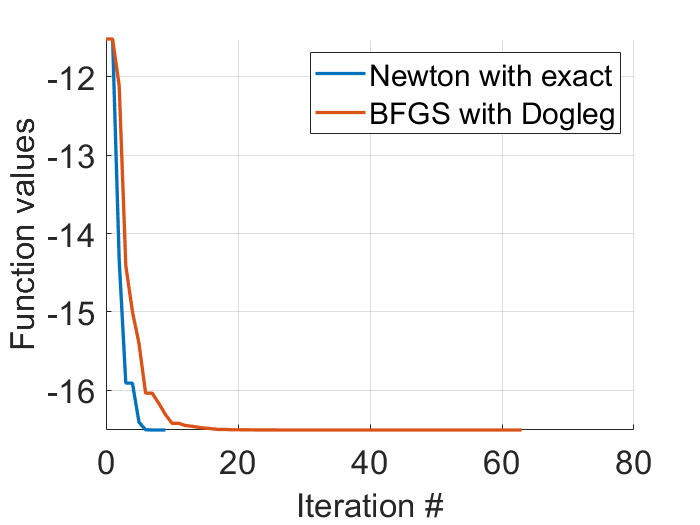
\includegraphics[width=\linewidth]{images/3-1-fun.png}
        \caption{}
        \label{fig4:a}
        \vspace{4ex}
    \end{subfigure}%%
    \begin{subfigure}[b]{0.5\linewidth}
        \centering
        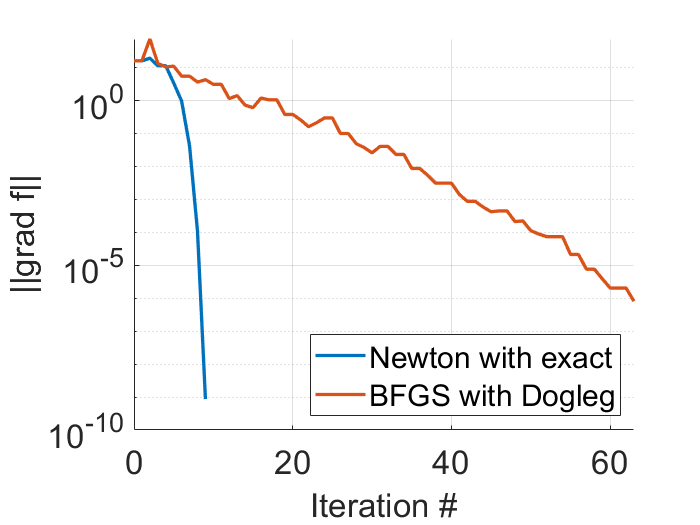
\includegraphics[width=\linewidth]{images/3-1-grad.png}
        \caption{}
        \label{fig4:b}
        \vspace{4ex}
    \end{subfigure}
    \caption{Function values of the Newton method with the exact solver and the BFGS method using the dogleg method at each iteration are shown in (a) while the norm of the gradient of the function value is shown in (b) when starting at the first initial condition.}
    \label{fig4}
\end{figure}
\begin{figure}[H]
    \begin{subfigure}[b]{0.5\linewidth}
        \centering
        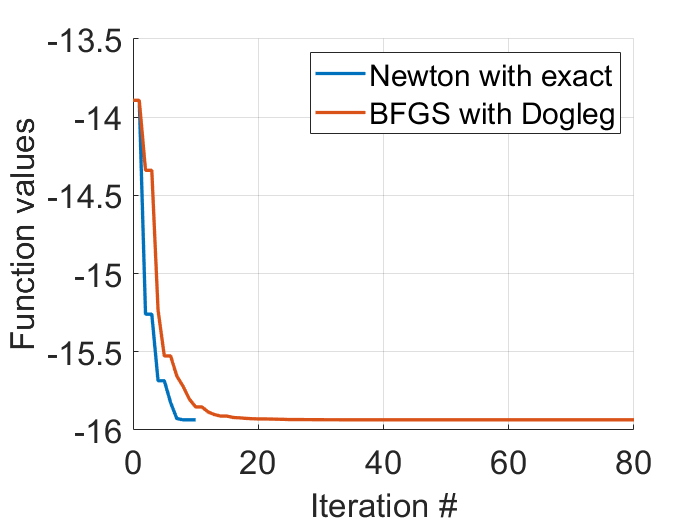
\includegraphics[width=\linewidth]{images/3-2-fun.png}
        \caption{}
        \label{fig5:a}
        \vspace{4ex}
    \end{subfigure}%%
    \begin{subfigure}[b]{0.5\linewidth}
        \centering
        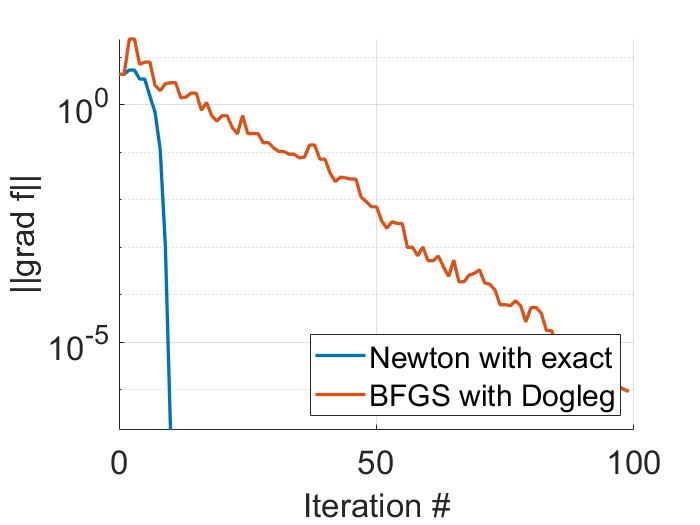
\includegraphics[width=\linewidth]{images/3-2-grad.png}
        \caption{}
        \label{fig5:b}
        \vspace{4ex}
    \end{subfigure}
    \caption{Function values of the Newton method with the exact solver and the BFGS method using the dogleg method at each iteration are shown in (a) while the norm of the gradient of the function value is shown in (b) when starting at the second initial condition.}
    \label{fig5}
\end{figure}
\begin{figure}[H]
    \begin{subfigure}[b]{0.5\linewidth}
        \centering
        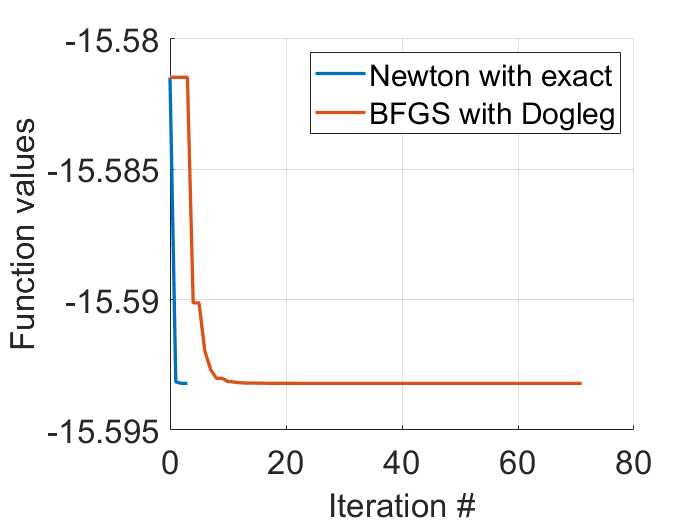
\includegraphics[width=\linewidth]{images/3-3-fun.png}
        \caption{}
        \label{fig6:a}
        \vspace{4ex}
    \end{subfigure}%%
    \begin{subfigure}[b]{0.5\linewidth}
        \centering
        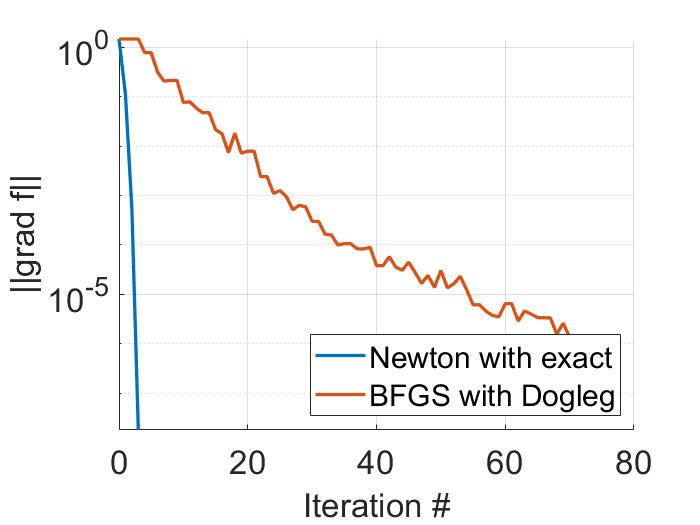
\includegraphics[width=\linewidth]{images/3-3-grad.png}
        \caption{}
        \label{fig6:b}
        \vspace{4ex}
    \end{subfigure}
    \caption{Function values of the Newton method with the exact solver and the BFGS method using the dogleg method at each iteration are shown in (a) while the norm of the gradient of the function value is shown in (b) when starting at the third initial condition.}
    \label{fig6}
\end{figure}
\begin{figure}[H]
    \begin{subfigure}[b]{0.5\linewidth}
        \centering
        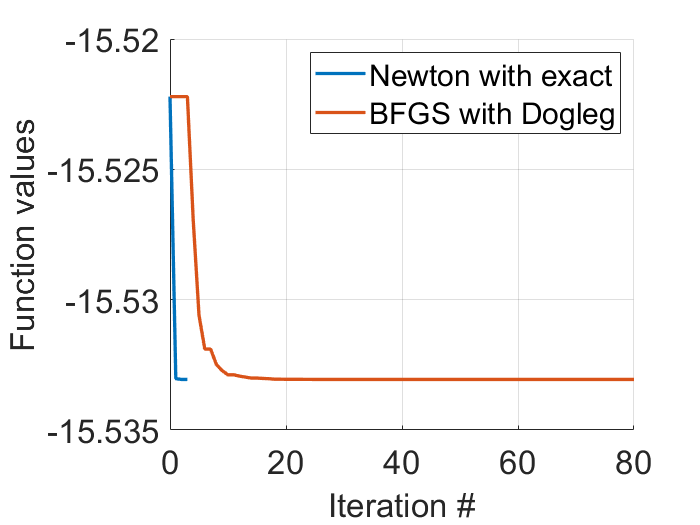
\includegraphics[width=\linewidth]{images/3-4-fun.png}
        \caption{}
        \label{fig7:a}
        \vspace{4ex}
    \end{subfigure}%%
    \begin{subfigure}[b]{0.5\linewidth}
        \centering
        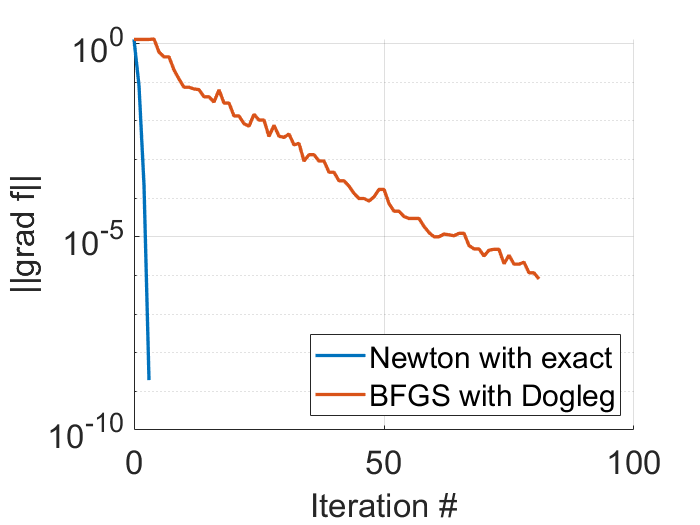
\includegraphics[width=\linewidth]{images/3-4-grad.png}
        \caption{}
        \label{fig7:b}
        \vspace{4ex}
    \end{subfigure}
    \caption{Function values of the Newton method with the exact solver and the BFGS method using the dogleg method at each iteration are shown in (a) while the norm of the gradient of the function value is shown in (b) when starting at the fourth initial condition.}
    \label{fig7}
\end{figure}
\begin{figure}[H]
    \begin{subfigure}[b]{0.5\linewidth}
        \centering
        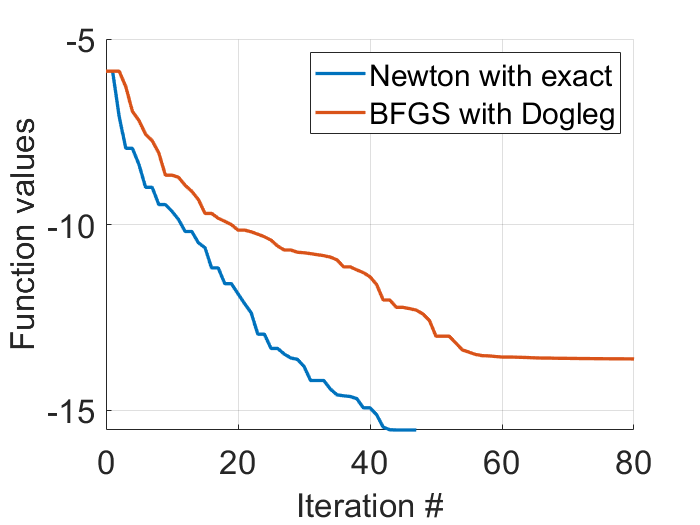
\includegraphics[width=\linewidth]{images/3-5-fun.png}
        \caption{}
        \label{fig8:a}
        \vspace{4ex}
    \end{subfigure}%%
    \begin{subfigure}[b]{0.5\linewidth}
        \centering
        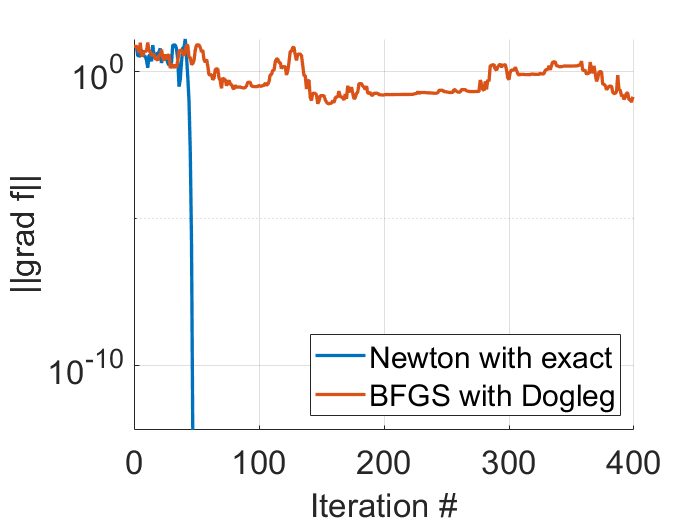
\includegraphics[width=\linewidth]{images/3-5-grad.png}
        \caption{}
        \label{fig8:b}
        \vspace{4ex}
    \end{subfigure}
    \caption{Function values of the Newton method with the exact solver and the BFGS method using the dogleg method at each iteration are shown in (a) while the norm of the gradient of the function value is shown in (b) when starting at a random initial condition.}
    \label{fig8}
\end{figure}


\end{proof}
\end{problem}




%---------------%
%---Problem 4---%
%---------------%


\begin{problem}%[vskip]
\subsection*{Problem 4}

(Approx. Problem 3.1 from [NW]) Write a code that applies the two algorithms from the previous problem (the trust-region BFGS with the dogleg solver and the trust-region Newton with the exact subspace solver) to the Rosenbrock function as in Problem 4 of HW9:
\[
    f (x, y) = 100(y - x^2)^2 + (1 - x)^2.
\]
Experiment with the same two initial conditions: $(1.2, 1.2) \and (-1.2, 1)$. Plot the level sets of the Rosenbrock function using the command contour and plot the iterations for each method over it. Plot $\norm{(x_k, y_k) - (x^*, y^*)}$ versus $k$ in the logarithmic scale along the $y$-axis for each method. Compare the performance of the methods.

\subsection*{Solution}
\begin{proof}
We begin by modifying the code we used above to find the minima of the Rosenbrock function. We begin the search from the initial conditions $(1.2,1.2)$ and $(-1.2,1)$ and plot the contour and the iterates upon it seen in Figures \ref{fig4-1} and \ref{fig4-2}. Next, we plot the $\norm{(x_k, y_k) - (x^*, y^*)}$ versus $k$ in the logarithmic scale along the $y$-axis as seen in Figures \ref{fig3}. We observe that Newton with the exact solver convergences in fewer iterations than the BFGS method using the dogleg solver. But both methods are able to identify the local minima.

My code used for this problem can be found at \url{https://github.com/MarvynBailly/AMSC660/tree/main/homework10}.

\begin{figure}[H]
    \begin{subfigure}[b]{0.5\linewidth}
        \centering
        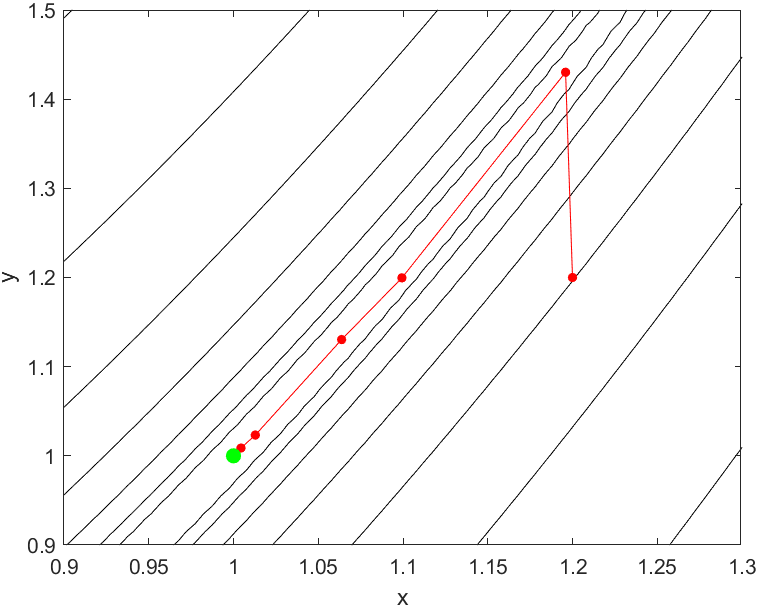
\includegraphics[width=\linewidth]{images/4-cont-N-1.2,1.2.png}
        \caption{Newton with exact subproblem solver.}
        \label{fig4-1:a}
        \vspace{4ex}
    \end{subfigure}%%
    \begin{subfigure}[b]{0.5\linewidth}
        \centering
        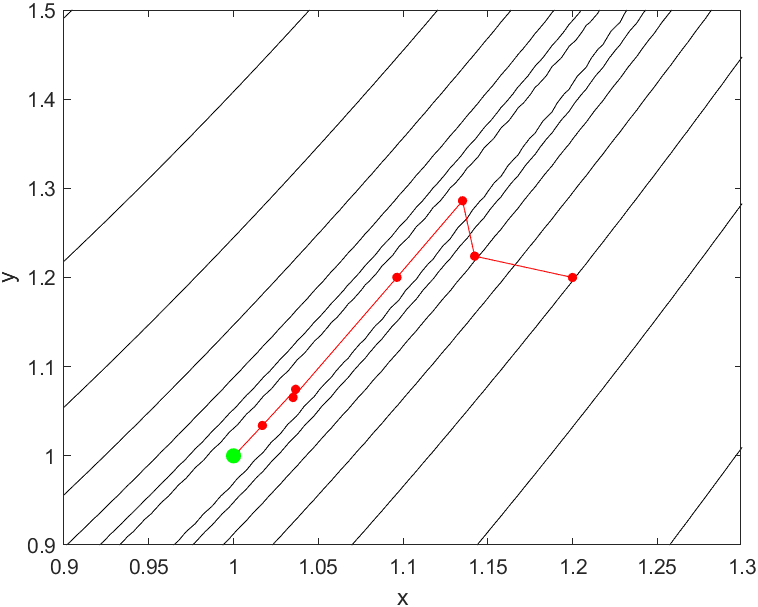
\includegraphics[width=\linewidth]{images/4-cont-BFGS-1.2,1.2.png}
        \caption{BFGS method with Dogleg subproblem solver.}
        \label{fig4-1:b}
        \vspace{4ex}
    \end{subfigure}
    \caption{A contour plot of the Rosenbrock function with iterates of the Newton method using the exact subproblem solver (seen in (a)) compared to the BFGS method using the Dogleg subproblem solver (seen in (b)) from the initial condition $(1.2,1.2)$}
    \label{fig4-1}
\end{figure}
\begin{figure}[H]
    \begin{subfigure}[b]{0.5\linewidth}
        \centering
        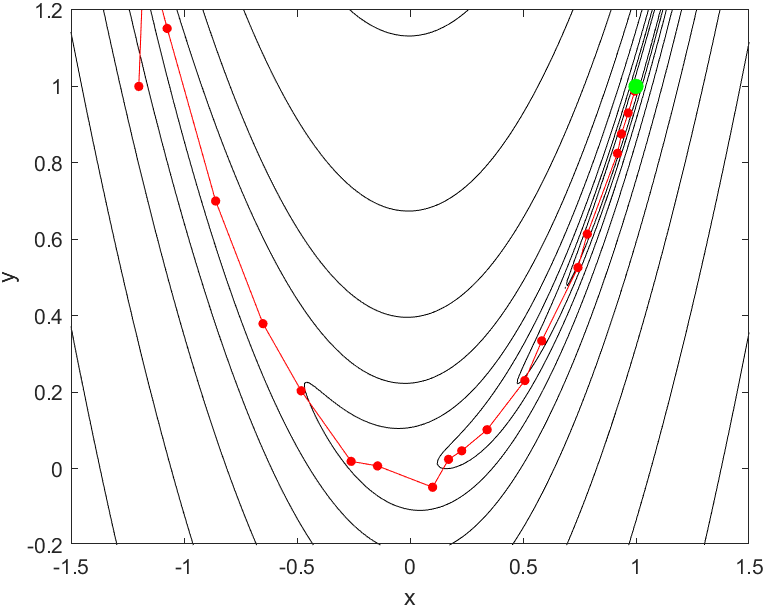
\includegraphics[width=\linewidth]{images/4-cont-N--1.2,1.png}
        \caption{Newton with exact subproblem solver.}
        \label{fig4-2:a}
        \vspace{4ex}
    \end{subfigure}%%
    \begin{subfigure}[b]{0.5\linewidth}
        \centering
        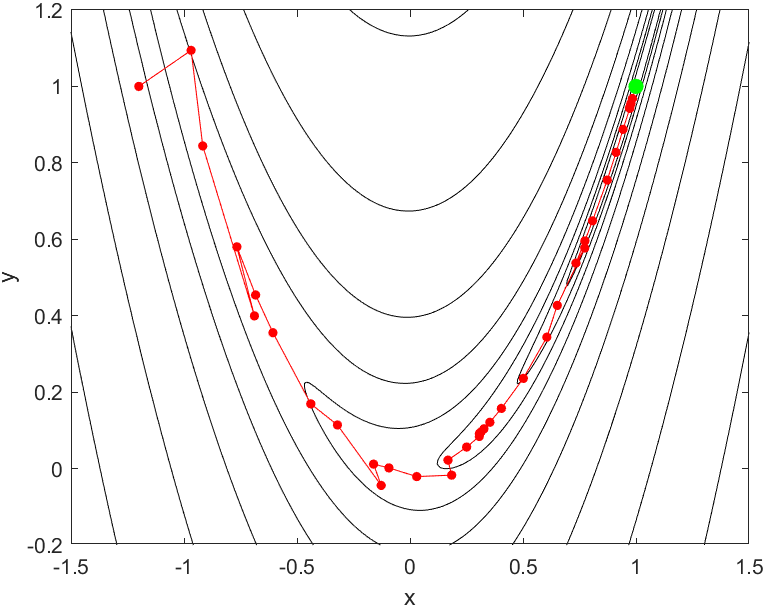
\includegraphics[width=\linewidth]{images/4-cont-BFGS--1.2,1.png}
        \caption{BFGS method with Dogleg subproblem solver.}
        \label{fig4-2:b}
        \vspace{4ex}
    \end{subfigure}
    \caption{A contour plot of the Rosenbrock function with iterates of the Newton method using the exact subproblem solver (seen in (a)) compared to the BFGS method using the Dogleg subproblem solver (seen in (b)) from the initial condition $(-1.2,1)$.}
    \label{fig4-2}
\end{figure}
\begin{figure}[H]
    \begin{subfigure}[b]{0.5\linewidth}
        \centering
        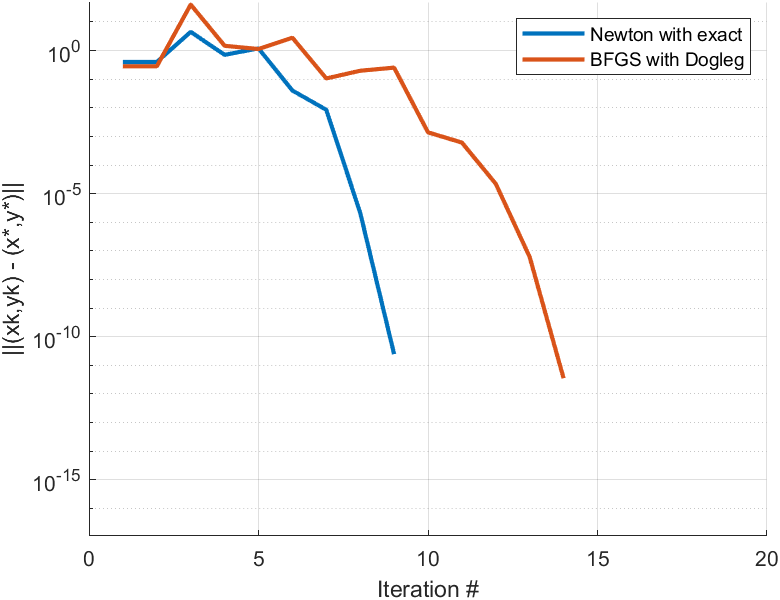
\includegraphics[width=\linewidth]{images/4-norm1.2,1.2.png}
        \caption{From initial condition $(1.2,1.2)$.}
        \label{fig3:a}
        \vspace{4ex}
    \end{subfigure}%%
    \begin{subfigure}[b]{0.5\linewidth}
        \centering
        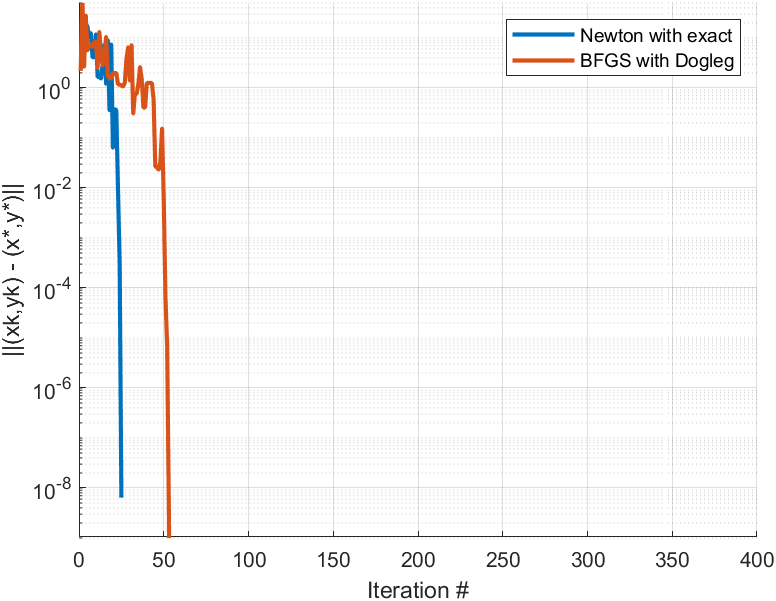
\includegraphics[width=\linewidth]{images/4-norm-1.2,1.png}
        \caption{From initial condition $(-1.2,1)$.}
        \label{fig3:b}
        \vspace{4ex}
    \end{subfigure}
    \caption{Plot of $\norm{(x_k, y_k) - (x^*, y^*)}$ versus $k$ in the logarithmic scale along the $y$-axis. The initial condition $(1.2,1.2)$ is shown in (a) while the initial condition $(-1.2,1)$ is shown in (b).}
    \label{fig3}
\end{figure}


\end{proof}
\end{problem}












\end{document}